\documentclass[a4paper,12pt,journal]{IEEEtran}
\usepackage[utf8]{inputenc}
\usepackage{tikz}
\title{Digital rotating clock}
\author{Nikolaj Iversen, Matthias Harald Hessels}

\newcommand{\ringwidth}{0.2}
\newcommand{\offA}{0.3}
\newcommand{\offB}{-0.5}

\begin{document}

\maketitle

\begin{abstract}
In this project a linear array of LED's, rotating at a high speed to simulate a display will be created.
The LED's will be mounted on a PCB which will act as an arm.
An FPGA will be used to keep track of the position of the arm and control which LED's should be turned on at that point in time.
The image to be displayed is an analog clock, so the image changes periodically and makes sense on a circular display.
\end{abstract}

\section{The LED PCB}
The PCB which will be rotating with the LED's is the main board.
The target is to drive 32 LED's placed in a straight line.

The LED's, transistors and resistors will be SMD components, in order to make the arm as small as possible and therefore as light as possible.

In order to turn the LED's on and off a communication with the LED's needs to be established.
The position of the arm must be known in order for the FPGA in order to make a stable image.
\subsection{Communication}
The board will be rotating, making the communication to this board a problem.
Existing solutions called slip rings exist, but the ones in the price range of this project is rated for 250 rpm, which will be too slow for this project.
So a custom solution will be devised to combat this.
By making a ring on the PCB, the wires going up to the board can be stationary and always keep contact to the ring.
This is assumed to work, but further testing of how well this performs on higher speeds will have to be tested.
Because this is assumed to be difficult to achieve, as few wires to the board as possible is wanted.

To turn a single LED on and off it requires a ground, a $V_+$ and signal.
Giving the board $32+2$ wires becomes impossible without making the board really big.
Instead a GPIO extender is used. 
Component $1016-1715-5-ND$ at digikey is chosen for this.
This requires a single I2C communication to give a 16 port output.
This reduces the communication to two signals, one clock signal, one ground and one $3.3V$ wire, 5 wires in total.
The I2C uses ID in the transmission, so both could be controlled with a single wire, but that would increase the number of packages needed to be sent.

\subsection{Position encoding}
To get information about the position of the arm, a magnet will be mounted the board and passing over several Hall sensors on the ground.
Three Hall sensors will be used in order to get a detailed view of where the arm is placed.
This can be used to estimate the speed of the arm keep timing constraints.
Hall sensors are available in the component storage, but ordered anyway as the system depends on those and it is not a usual component to be in stock all the time.

\section{Motor}
The motor chosen for this project is a DC motor capable of a high speed.
$50Hz$ refresh time is used for regular displays. 
The flickering is often visible, as light sources flicker at the same speed, so this is seen as a minimum.
$50Hz$ requires a speed of $3000$ RPM.
Component $2457411$ at Farnell is a DC motor which can move at $9000$ RPM with a $6V$ source.
This means the motor can be driven with a PWM signal and be kept below the ratings if needed.
$9000$ RPM means the arm will make up to 150 revolutions per second.
1 revolution takes $6666.6 \mu s$
If the control is $\frac{1}{60}$ of a revolution, the time to send the I2C signal is $111.1 \mu s$.
A complete signal is $30$ bits so a minimum of 270 kHz is needed.
The IO expander can operate up to 400 kHz making this possible.

\section{Ring Connector}
\begin{figure}
    \centering
    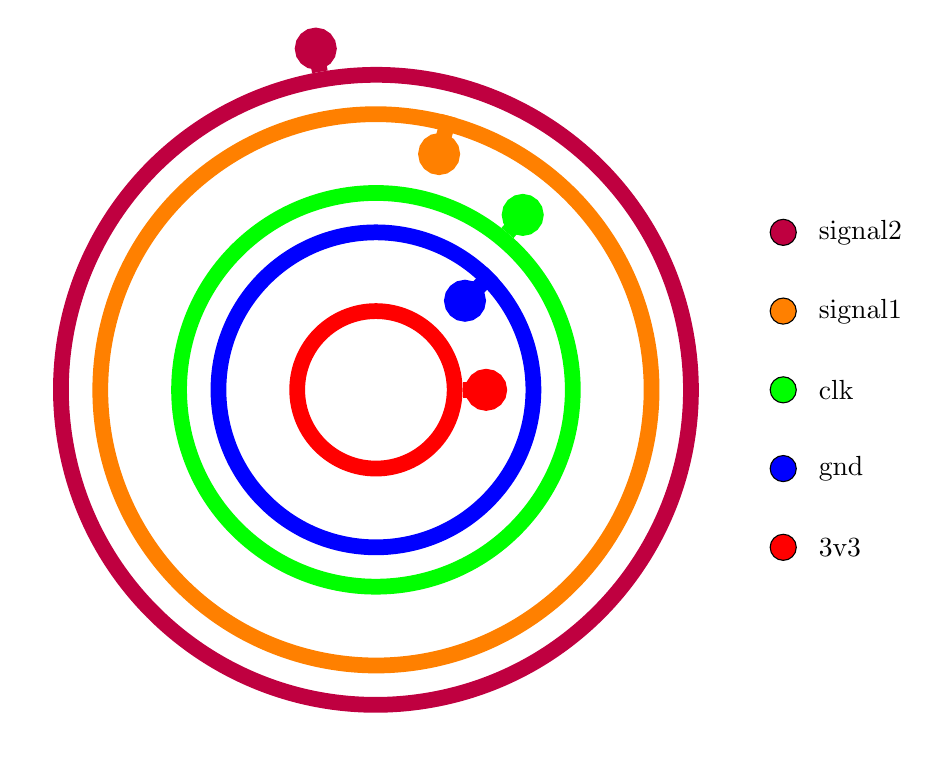
\begin{tikzpicture}[node distance=2cm]
        %rings
        \node[draw, circle, line width=\ringwidth cm, rotate=0  ,  color = red    , minimum width=2.0cm, name=3v3    ] at (0,0) {}; 
        \node[draw, circle, line width=\ringwidth cm, rotate=45 ,  color = blue   , minimum width=4.0cm, name=gnd    ] at (0,0) {}; 
        \node[draw, circle, line width=\ringwidth cm, rotate=50 ,  color = green  , minimum width=5.0cm, name=clk    ] at (0,0) {}; 
        \node[draw, circle, line width=\ringwidth cm, rotate=75 ,  color = orange , minimum width=7.0cm, name=signal1] at (0,0) {}; 
        \node[draw, circle, line width=\ringwidth cm, rotate=100,  color = purple , minimum width=8.0cm, name=signal2] at (0,0) {}; 
        
        %pads
        \draw[red    , line width=\ringwidth cm, rotate=0  ]     (3v3.0) -- ++(\offA,0) node[draw, circle, fill= red    , minimum width=0.25cm] {};
        \draw[blue   , line width=\ringwidth cm, rotate=45 ]     (gnd.0) -- ++(\offB,0) node[draw, circle, fill= blue   , minimum width=0.25cm] {};
        \draw[green  , line width=\ringwidth cm, rotate=50 ]     (clk.0) -- ++(\offA,0) node[draw, circle, fill= green  , minimum width=0.25cm] {};
        \draw[orange , line width=\ringwidth cm, rotate=75 ] (signal1.0) -- ++(\offB,0) node[draw, circle, fill= orange , minimum width=0.25cm] {};
        \draw[purple , line width=\ringwidth cm, rotate=100] (signal2.0) -- ++(\offA,0) node[draw, circle, fill= purple , minimum width=0.25cm] {};
        
        %legend
        \draw 
        (0,0) ++( 5  ,-2) node[draw, circle, right, fill = red   ] {} ++(0.5,0) node[right] {3v3    }
              ++(-0.5, 1) node[draw, circle, right, fill = blue  ] {} ++(0.5,0) node[right] {gnd    }
              ++(-0.5, 1) node[draw, circle, right, fill = green ] {} ++(0.5,0) node[right] {clk    }
              ++(-0.5, 1) node[draw, circle, right, fill = orange] {} ++(0.5,0) node[right] {signal1}
              ++(-0.5, 1) node[draw, circle, right, fill = purple] {} ++(0.5,0) node[right] {signal2}
        ;
    \end{tikzpicture}
    \caption{Sketch of the schematic side of the slip ring.}
\end{figure}


\end{document}
